\chapter{Результаты проектирования системы Интеллектуального ассистента врача щитовидной железы}

\section{Разработка микросервисной архитектуры системы}

\subsection{Паттерн API Composition}
Каждому спроектированному компоненту системы соответствует свой микросервис. Общение между микросервисами осуществляется 
синхронным и асинхронным способом. Однако в распределенных системах следует избегать лишних зависимостей между микросервисами, это
может повлеч за собой сложности в масштабировании и обслуживании системы, проблемы с каскадными ретраями, и в целом делает изолированный и
обособленные части системы зависимыми от других частей системы.\\
Для удовлетворения требовани о регистрации пользователей системы нам требуется сообщить информацию о новом пользователе в 2 компонента:
компоненту авторизации и аутентификации и компоненту управления пользователями.\\
Для избежания лишней зависимости между компонентами, мы используем паттерн Composition-API. API Composition паттерн 
— это подход в архитектуре микросервисов, который позволяет выносить логику взаимодействия между микросервисами в отдельный сервис более верхнего уровня.

\begin{figure}[H]%
	\begin{center}
		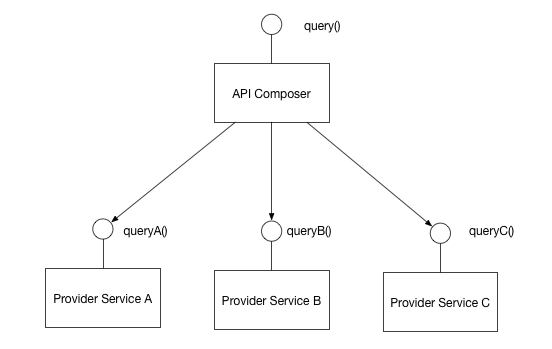
\includegraphics[width=.6\columnwidth]{./img/new/api_composition_pattern.png}%
	\end{center}
	\caption{API Composition паттерн}%
	\label{pic:api_composition_pattern}%
\end{figure}

\subsection{Способы взаимодействия между микросервисами}
Основные запросы которые будут поступать в ИИ ассистент врача, это запросы на получение того или иного ресурса. Данные запросы
реализуются посредством обычных синхронных интернет запросов, в API Composition. Далее из API Composition запросы передаются в микросервисы.


Однако стоит рассмотреть сценарий загрузки узи снимков на обработку в систему. Обработка узи снимка занимает значительное для пользователя время.
Нужен механизм, который избавит пользователя от необходимости активного ожидания результатов обработки узи снимка.\\
Решением этой проблемы - во время загрузки узи снимка, система ставит асинхронную задачу на обработку узи снимка. Если 
задача поставлена успешно, пользователь получает идентификатор задачи, после чего может посредством отдельных запросов узнать статус задачи.
В данном случае ожидание пользователя будет сведено к загрузке узи снимка.
В таком случае, схема начала обработки узи снимка будет выглядеть следующим образом:
\begin{figure}[H]%
	\begin{center}
		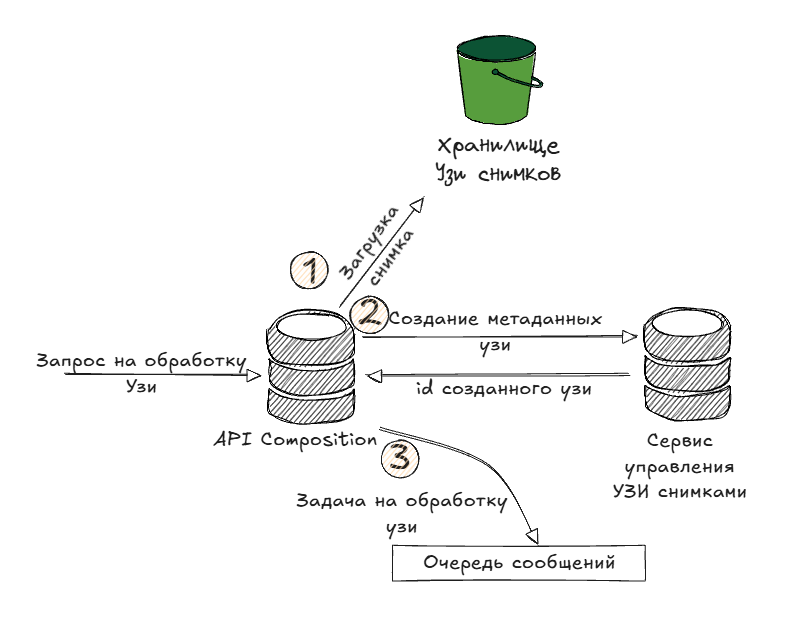
\includegraphics[width=.6\columnwidth]{./img/new/async.png}%
	\end{center}
	\caption{Схема асинхронной обработки узи снимка}%
	\label{pic:async}%
\end{figure}

\subsection{Итоговая архитектура системы Интеллектуального ассистента врача щитовидной железы}

Применяя паттерны API Composition при проектировании, а также учитывая синхронное и асинхронное взаимодействие между микросервисами,
мы получаем следующую архитектуру системы:
\begin{figure}[H]%
	\begin{center}
		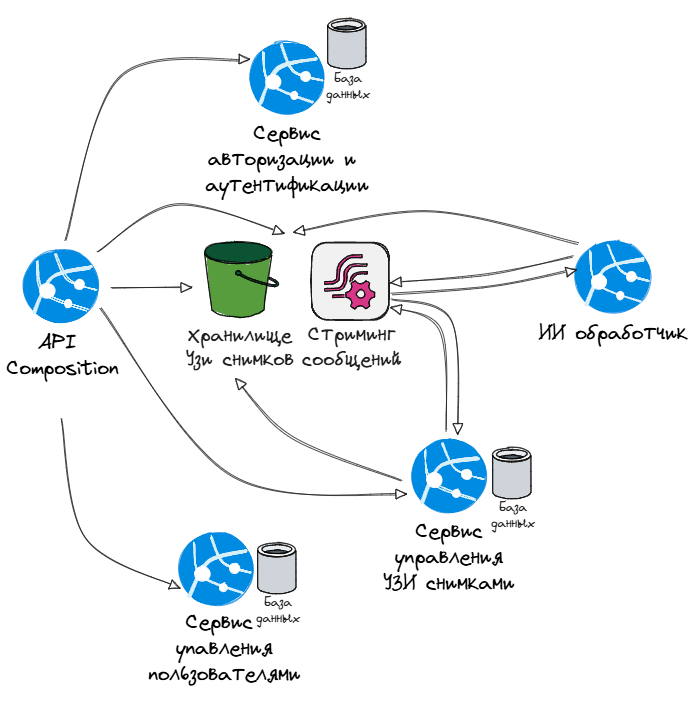
\includegraphics[width=.6\columnwidth]{./img/new/microservice_arch.png}%
	\end{center}
	\caption{Итоговая архитектура микросервисной системы}%
	\label{pic:microservice_arch}%
\end{figure}

\section{Выбор технологий и инструментов для технической реализации системы}

\subsection{Выбор языка программирования}
\subsection{Реляционные хранилища данных}
\textbf{Реляционные базы данных}: Реляционные базы данных, такие как MySQL и PostgreSQL, предлагают структурированный способ хранения данных с использованием таблиц, что позволяет легко реализовать связи между ними. Они подходят для большинства приложений, требующих согласованности и целостности данных.

\textbf{Описание реляционных баз данных}

1. \textbf{MySQL}:
   - \textbf{Описание}: MySQL — это популярная реляционная база данных с открытым исходным кодом, которая используется во множестве веб-приложений и сервисов. Она известна своей производительностью, простотой настройки и широким сообществом.
   - \textbf{Назначение}: Широко используется для веб-приложений, особенно тех, которые требуют быстрого доступа к данным.

2. \textbf{PostgreSQL}:
   - \textbf{Описание}: PostgreSQL — это мощная объектно-реляционная база данных с открытым исходным кодом, которая поддерживает различные типы данных и расширенные функции, такие как работа с JSON и поиск по полнотекстовому содержимому.
   - \textbf{Назначение}: Подходит для сложных и крупных приложений, требующих расширенной функциональности обработки данных.


\textbf{Сравнение MySQL и PostgreSQL}
Ниже представлено сравнение преимуществ и недостатков MySQL и PostgreSQL.

\begin{table}[h]
    \centering
    \begin{tabular}{|l|l|l|}
        \hline
        \textbf{Система}            & \textbf{Преимущества}                          & \textbf{Недостатки}                                \\ \hline
        \textbf{MySQL}              & - Высокая производительность                   & - Ограниченная поддержка сложных запросов       \\ \hline
                                   & - Простота настройки                           & - Менее гибкая работа с типами данных            \\ \hline
                                   & - Широкое сообщество и поддержка              & - Нет полной поддержки ACID в некоторых режимах  \\ \hline
        \textbf{PostgreSQL}        & - Поддержка сложных запросов и индексов       & - Меньшая производительность для простых операций   \\ \hline
                                   & - Расширенные функции для работы с данными    & - Сложнее в настройке и администрировании        \\ \hline
                                   & - Полная поддержка ACID и транзакций          &                                                  \\ \hline
    \end{tabular}
    \caption{Сравнение MySQL и PostgreSQL}
\end{table}

\textbf{Заключение}

Учитывая наши требования и специфику приложений, мы выбираем PostgreSQL как основное решение для хранения данных в нашей архитектуре.
\subsection{Хранилище УЗИ снимков}

\subsection{Синхронное взаимодействие между микросервисами}

Микросервисы могут синхронно общаться между собой с использованием различных технологий и протоколов. 
В этом контексте рассмотрим четыре популярных метода взаимодействия: HTTP/REST API, gRPC, GraphQL и WebSocket.

В большинстве случаев для микросервисов, которые обмениваются фиксированными данными, использование GraphQL 
может быть излишним, поскольку этот подход предназначен для динамического запроса данных. В сценариях, 
где структуры данных заранее известны и не требуют изменения, REST API будет более простым и 
понятным решением. То же касается и WebSocket: двунаправленный стриминг данных может быть избыточным для 
многих бизнес-приложений, где достаточно стандартного запроса и ответа.

Таким образом, основные методы, которые стоит рассмотреть для синхронного взаимодействия микросервисов, — 
это HTTP/REST API и gRPC.


\textbf{HTTP/REST API}
HTTP/REST API — это один из самых распространенных способов синхронного взаимодействия между микросервисами. Каждый микросервис предоставляет набор эндпоинтов, к которым другие сервисы могут обращаться для выполнения операций и получения данных. Используя стандартные методы HTTP (GET, POST, PUT, DELETE), микросервисы обмениваются сообщениями с четко определенными правилами и структурой.


\textbf{Преимущества использования HTTP/REST}
\begin{itemize}
    \item \textbf{Простота}: REST API легко реализовать и документировать. Он основан на понятных стандартах HTTP и может использоваться практически на любой платформе.
    \item \textbf{Читаемость}: Структура URL и использование HTTP-методов делают интерфейс API интуитивно понятным и удобным для работы разработчиков.
    \item \textbf{Совместимость}: REST API может легко взаимодействовать с разными языками программирования и платформами, что делает его универсальным решением для микросервисной архитектуры.
\end{itemize}


\textbf{gRPC}
gRPC, разработанный Google, представляет собой высокопроизводительный фреймворк для удаленных вызовов процедур (RPC), который поддерживает множество языков программирования. Он использует HTTP/2 для передачи данных, что обеспечивает преимущества, такие как многопоточность и меньшие задержки при передаче информации.


\textbf{Преимущества использования gRPC}
\begin{itemize}
    \item \textbf{Производительность}: Использование HTTP/2 позволяет gRPC эффективно обрабатывать множество параллельных запросов, что делает его более производительным, чем традиционные REST API.
    \item \textbf{Статическая типизация}: gRPC использует Protocol Buffers для описания структуры данных, что позволяет разработчикам строго определять, какой тип данных будет передаваться. Это обеспечивает дополнительную безопасность и позволяет избежать ошибок при взаимодействии между сервисами.
    \item \textbf{Автогенерация кода}: Удобство разработки достигается благодаря автоматической генерации клиентского кода на разных языках, что ускоряет процесс создания микросервисов.
\end{itemize}


\textbf{Сравнение HTTP/REST API и gRPC}
\begin{table}[h]
    \centering
    \begin{tabular}{|l|l|l|}
        \hline
        \textbf{Характеристика}           & \textbf{HTTP/REST API}                          & \textbf{gRPC}                                     \\ \hline
        Протокол                  & Основан на HTTP/1.1 или HTTP/2            & Использует HTTP/2                             \\ \hline
        Структура данных          & Ограничена JSON/XML                        & Использует Protocol Buffers для сериализации \\ \hline
        Типизация                 & Нестатическая типизация (JSON)            & Статическая типизация (протоколы определены) \\ \hline
        Производительность         & Может иметь более высокую задержку         & Обычно низкая задержка, высокая производительность \\ \hline
        Поддержка потоковой передачи & Ограниченная                                & Поддерживает стриминг (односторонний и двунаправленный) \\ \hline
        Автогенерация клиента     & Обычно требует ручного создания клиентского кода & Генерация клиентского кода на многих языках из .proto-файлов \\ \hline
        Простота и читаемость     & Прост в реализации, легко понимается      & Требует понимания Protocol Buffers и gRPC, может быть сложнее для освоения \\ \hline
        Универсальность           & Широко используется и поддерживается, совместим с многими технологиями & Хорошо подходит для систем с высокой нагрузкой, но менее распространен \\ \hline
        Тестирование и отладка   & Легче тестировать с инструментами для работы с HTTP (например, Postman) & Может потребоваться больше усилий для настройки инструментов тестирования \\ \hline
    \end{tabular}
    \caption{Сравнение HTTP/REST API и gRPC}
\end{table}


\textbf{Заключение}
Нашей системе не требуется возможность динамической типизации, поэтому выбор сделать в сторону gRPC.

\subsection{Асинхронное взаимодействие} % kafka

Асинхронное взаимодействие между микросервисами позволяет увеличить производительность и гибкость распределенных систем. В этом подходе микросервисы могут обмениваться данными без необходимости дожидаться ответа, что снижает задержки и повышает общую эффективность системы. Рассмотрим основные методы асинхронного взаимодействия.

\textbf{Основные методы асинхронного взаимодействия}
\begin{itemize}
    \item \textbf{Очереди сообщений}: Использование систем обмена сообщениями, таких как RabbitMQ, Apache Kafka или Redpanda, позволяет отправлять сообщения между микросервисами без прямого связывания. Один сервис может отправлять сообщения в очередь, а другой — извлекать их и обрабатывать по мере возможности. Это гарантирует, что сервисы могут работать независимо друг от друга и не блокируют друг друга в случае высокой нагрузки.
    \item \textbf{Событийно-ориентированная архитектура}: В этой архитектуре микросервисы реагируют на события, происходящие в системе. События могут генерироваться различными компонентами и служить сигналами для других микросервисов о том, что произошло что-то важное (например, изменение состояния, завершение задачи и т. д.). Это позволяет строить более гибкие и масштабируемые системы.
    \item \textbf{HTTP-события (Webhooks)}: Использование вебхуков позволяет микросервису отправлять HTTP-запросы в другие сервисы при наступлении определённых событий. Это простой способ интеграции, позволяющий уведомлять другие службы о произошедших изменениях или событиях.
\end{itemize}

Выбор в сторону очередей сообщений также обуславливается необходимостью наличия механизма Dead Letter Queue (DLQ), который позволяет обрабатывать ошибки при отправке и получении сообщений. Кроме того, мы стремимся автоматизировать хранение сообщений, что делает использование очередей сообщений предпочтительным решением.

\textbf{Описание систем очередей сообщений}
\begin{itemize}
    \item \textbf{Apache Kafka}:
            - Kafka — это распределенная платформа для потоковой передачи данных, которая обеспечивает высокую пропускную способность и низкую задержку. Она работает по принципу публикации и подписки, позволяя множеству клиентов читать и писать сообщения.
            - \textbf{Назначение}: Идеально подходит для обработки потоков данных в реальном времени и хранения больших объемов событий с возможностью их долговременного хранения.
    \item \textbf{Redpanda}:
            - Redpanda — это высокопроизводительная, совместимая с Kafka, распределенная система сообщений, оптимизированная для работы с потоками данных в реальном времени.
            - \textbf{Назначение}: Обеспечивает низкую задержку и простоту настройки, что делает её предпочтительной для решений, требующих высокой производительности. 
    \item \textbf{Apache Pulsar}:
            - Pulsar — это распределенная система потоковой передачи данных, которая поддерживает многопоточность и управление потоками. Она предоставляет гибкий подход к очередям сообщений и событиям.
            - \textbf{Назначение}: Отличается поддержкой долгосрочного хранения сообщений и сложных сценариев работы с геораспределёнными данными.
\end{itemize}



\textbf{Сравнение систем очередей сообщений}
Ниже представлено сравнение преимуществ и недостатков Apache Kafka, Redpanda и Apache Pulsar.

\begin{table}[h]
    \centering
    \begin{tabular}{|l|l|l|}
        \hline
        \textbf{Система}            & \textbf{Преимущества}                          & \textbf{Недостатки}                                \\ \hline
        \textbf{Apache Kafka}       & - Высокая надежность                    & - Сложность настройки и администрирования     \\ \hline
                                   & - Масштабируемость                       & - Требует дополнительных ресурсов              \\ \hline
                                   & - Долговременное хранение данных         & - Зависимость от Zookeeper                      \\ \hline
        \textbf{Redpanda}           & - Низкая задержка                        & - Меньшая экосистема поддержки                 \\ \hline
                                   & - Простота настройки                     &                                                \\ \hline
                                   & - Совместимость с Kafka                 &                                                \\ \hline
        \textbf{Apache Pulsar}      & - Гибкость                               & - Сложность архитектуры и настройки            \\ \hline
                                   & - Поддержка геораспределённых данных    & - Меньшая популярность по сравнению с Kafka    \\ \hline
                                   & - Высокая масштабируемость              &                                                \\ \hline
    \end{tabular}
    \caption{Сравнение систем очередей сообщений}
\end{table}

\textbf{Заключение}
Асинхронное взаимодействие, организованное через очереди сообщений, является эффективным способом повышения производительности и устойчивости микросервисов. Учитывая возможности по снижению задержки и простой настройке, мы выбрали Redpanda как предпочтительное решение для организации асинхронного взаимодействия между микросервисами.

\subsection{Выбор системы контроля версий}
\subsection{Выбор системы сборки приложения}
\subsection{Выбор системы контейнеризации}

\section{Выводы}

В результате были спроектированы модули системы и правила их взаимодействия с учетом выбранных средств разработки
на этапе анализа.

% В этой главе описывается, что и как было спроектировано. 
% При необходимости, описывается использованная методика проектирования. 
% Сюда же относится описание внешних и внутренних программных интерфейсов, 
% а также форматы и структуры входных и выходных данных.


% \section{Использование методики <<такой-то>> для проектирования программных систем <<такого-то типа>>}

% \dots

% \section{Общая архитектура системы \dots}

% \dots


% Команда \texorpdfstring необходима, чтобы программа просмотра PDF документов
% верно отображала текст формул в панели оглавления.
% При отсутствии команды \texorpdfstring там, где она необходима, LaTeX выводит
% предупреждение "Token not allowed in a PDF string"
% \section{Архитектура подсистемы \texorpdfstring{$1$}{1}\dots}

% \dots


% \section{Архитектура подсистемы \texorpdfstring{$N$}{N}\dots}

% \dots


% \section{
%   Проектирование протокола взаимодействия подсистем \texorpdfstring{$X$}{X} и
%   \texorpdfstring{$Y$}{Y}
% }

% \dots


% \section{Выводы}

% Следует перечислить, какие инженерные результаты были получены, а именно: 
% какие программные системы, подсистемы или модули были спроектированы. Следует 
% не только назвать полученные архитектуры, но и отметить их отличительные 
% особенности.

%%% Local Variables:
%%% TeX-engine: xetex
%%% eval: (setq-local TeX-master (concat "../" (seq-find (-cut string-match ".*-3-pz\.tex$" <>) (directory-files ".."))))
%%% End:
